\documentclass{article}

% set font encoding for PDFLaTeX or XeLaTeX
\usepackage{ifxetex}
\ifxetex
  \usepackage{fontspec}
\else
  \usepackage[T1]{fontenc}
  \usepackage[utf8]{inputenc}
  \usepackage{lmodern}
  \usepackage{graphicx}
\fi

% used in maketitle
\title{Actividad 6}
\author{Jesús Adrián Zatarain Alvarado}

% Enable SageTeX to run SageMath code right inside this LaTeX file.
% documentation: http://mirrors.ctan.org/macros/latex/contrib/sagetex/sagetexpackage.pdf
% \usepackage{sagetex}

\begin{document}
\maketitle

\section{Introducción}

En esta actividad se contunuará con la profundización en el lenguaje Python. En las anteriores actividades se trabajó con las capacidades que tenía para realizar gráficas, las cuales se realizaban con suma facilidad. En esta ocasión se pretende trabajar con sus funcionalidades numéricas, las cuales sirven para facilitar la recolección de datos y su posterior cálculo que resulta tedioso por la cantidad que se tienen que realizar.

Se incluye una síntesis de las secciones 1 y 2 del artículo de Fay and Graham que serań necesarias para realizar la actividad posterior.

Se anexarán todos los pasos de las actividades propuestas junto con su respectivos códigos y resultados obtenidos.

\section{Síntesis}

El artículo trata sobre la ley de Hooke para los sistemas de resortes. En cada una se ven varias situaciones que existen al estudiar estos sistemas. Se especializa especialmente en los sistemas de dos resortes conectados cada uno a una masa de manera que uno está seguido del otro y colgados.

En la primera sección se hace presencia de las ecuaciones diferenciales, y su uso en este caso para la modelación de sistemas de resortes acoplados. Existe un problema, al estar dos resortes acoplados a dos masas, uno seguido del otro, su descripción es mediante una ecución lineal de segundo orden para cada uno. Con unos arreglos pueden ser mostradas como ecuaciones diferenciales de cuarto orden ambos. También menciona que la solución del problemas puede llevar a la solución de sistemas de resortes con más elementos acoplados.

En la siguiente parte se enfoca en el modelaje de resortes acoplados, que consisten en dos resortes con conectados a dos masas en linea, uno seguido del otro. En esta sección hay cuatro ejemplos que son los que se tratarán en la actividad de la semana.

Cada resorte tiene asociado ciertas cantidades, tales como su constante, las masas acopladas y condiciones iniciales. En la sección se trabaja con la ley de Hooke para poder resumir el comportamiento de dos resortes en una ecuación que relaciona las cantidades anteriormente mencionadas.

El primer ejemplo fue práctico, para ilustrar esta idea y ver el comportamiento de estos dos resortes en una posterior gráfica. Hasta el ejemplo tres se vio un comportamiento lineal en los ejemplos donde sólo cambiaban sus amplitudes y fases. Pero en el cuarto se noto un comportamiento más errático .



\section{Actividad-código}

Para empezar, se mostró un ejemplo. Donde, en primera instancia, se especifican las variables a incluir a lo largo del programa y la definición de f. 

\begin{verbatim}
def vectorfield(w, t, p):
    """
    Defines the differential equations for the coupled spring-mass system.

    Arguments:
        w :  vector of the state variables:
                  w = [x1,y1,x2,y2]
        t :  time
        p :  vector of the parameters:
                  p = [m1,m2,k1,k2,L1,L2,b1,b2]
    """
    x1, y1, x2, y2 = w
    m1, m2, k1, k2, L1, L2, b1, b2 = p

    # Create f = (x1',y1',x2',y2'):
    f = [y1,
         (-b1 * y1 - k1 * (x1 - L1) + k2 * (x2 - x1 - L2)) / m1,
         y2,
         (-b2 * y2 - k2 * (x2 - x1 - L2)) / m2]
    return f
\end{verbatim}

En seguida se les da el valor deseado a cada parámetro relacionado con la elongación de los dos resortes. A la vez, que las regulaciones que va a tener el programa para realizar sus cálculos.

\begin{verbatim}
# Use ODEINT to solve the differential equations defined by the vector field
from scipy.integrate import odeint

# Parameter values
# Masses:
m1 = 1.0
m2 = 1.5
# Spring constants
k1 = 8.0
k2 = 40.0
# Natural lengths
L1 = 0.5
L2 = 1.0
# Friction coefficients
b1 = 0.8
b2 = 0.5

# Initial conditions
# x1 and x2 are the initial displacements; y1 and y2 are the initial velocities
x1 = 0.5
y1 = 0.0
x2 = 2.25
y2 = 0.0

# ODE solver parameters
abserr = 1.0e-8
relerr = 1.0e-6
stoptime = 10.0
numpoints = 250

# Create the time samples for the output of the ODE solver.
# I use a large number of points, only because I want to make
# a plot of the solution that looks nice.
t = [stoptime * float(i) / (numpoints - 1) for i in range(numpoints)]

# Pack up the parameters and initial conditions:
p = [m1, m2, k1, k2, L1, L2, b1, b2]
w0 = [x1, y1, x2, y2]

# Call the ODE solver.
wsol = odeint(vectorfield, w0, t, args=(p,),
              atol=abserr, rtol=relerr)

with open('two_springs.dat', 'w') as f:
    # Print & save the solution.
    for t1, w1 in zip(t, wsol):
        print (t1, w1[0], w1[1], w1[2], w1[3], file=f)
\end{verbatim}
 
 Que genera un archivo con una gran cantidad de valores acerca de los parámetros del sistema de resortes.
 
\begin{center}
  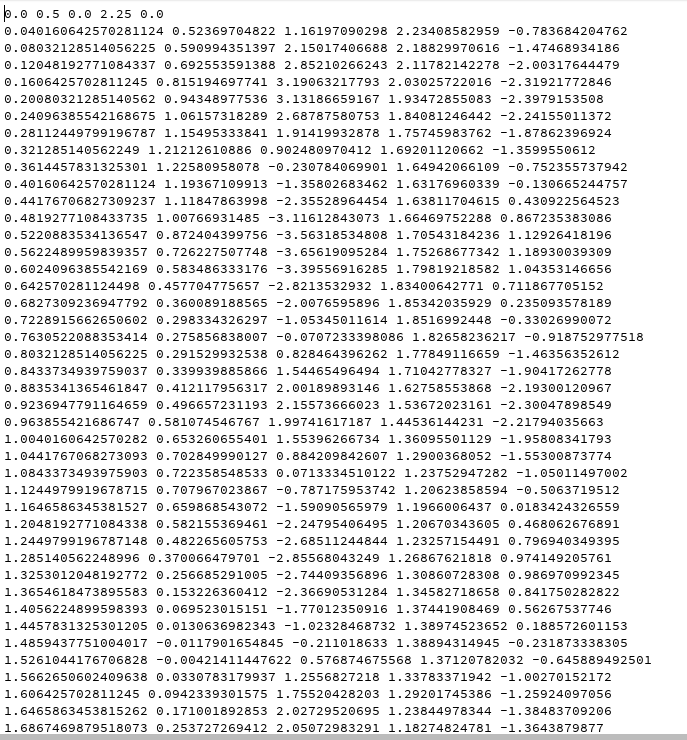
\includegraphics[width=6cm, height=6cm]{ejdat.png}
\end{center}

Lo siguiente es la graficación de los archivos generados. La gráfica debe mostrar el desplazamiento de las masas acopladas del sistema masa-resorte

\begin{verbatim}
  # Plot the solution that was generated

from numpy import loadtxt
from pylab import figure, plot, xlabel, grid, hold, legend, title, savefig
from matplotlib.font_manager import FontProperties

t, x1, xy, x2, y2 = loadtxt('two_springs.dat', unpack=True)

figure(1, figsize=(6, 4.5))

xlabel('t')
grid(True)
#hold(True)
lw = 1

plot(t, x1, 'b', linewidth=lw)
plot(t, x2, 'g', linewidth=lw)

legend((r'$x_1$', r'$x_2$'), prop=FontProperties(size=16))
title('Mass Displacements for the\nCoupled Spring-Mass System')
savefig('two_springs.png', dpi=100)
\end{verbatim}

\begin{center}
  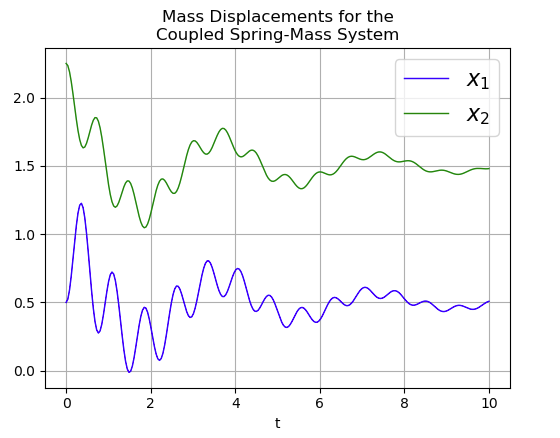
\includegraphics[width=6cm, height=6cm]{ejgraf.png}
\end{center}

\subsection{Ejemplo 2.1}

En este ejemplo es parecido al anterior, sólo que se le cambian ciertos parámetros 
Se inició igual, con los mismos parámetros, pero se modificaron los valores y la ecuación a resolver por el sistema.

\begin{center}
  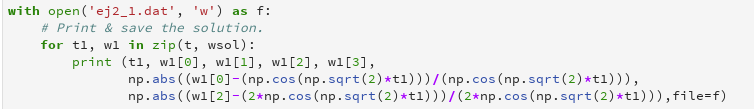
\includegraphics[width=6cm, height=6cm]{dat1.png}
\end{center}

\begin{center}
  \includegraphics[width=6cm, height=6cm]{dat.png}
\end{center}

\begin{verbatim}

# Plot the solution that was generated

import matplotlib.pyplot as plt
from numpy import loadtxt
from pylab import figure, plot, xlabel, grid, hold, legend, title, savefig
from matplotlib.font_manager import FontProperties
% matplotlib inline

t, x1, xy, x2, y2, e1,e2 = loadtxt('ej2_1.dat', unpack=True)

figure(1, figsize=(6, 4.5))

xlabel('t')
grid(True)
#hold(True)
lw = 1
plt.xlim(0,50)
plt.ylim (-2.5,2.5)

plot(t, x1, 'b', linewidth=lw)
plot(t, x2, 'g', linewidth=lw)

legend((r'$x_1$', r'$x_2$'), prop=FontProperties(size=16))
title('Plot of x1 and x2 showing synchronized motion')
savefig('ej2_1.1.png', dpi=100)
\end{verbatim}

que realiza la siguiente gráfica

\begin{center}
  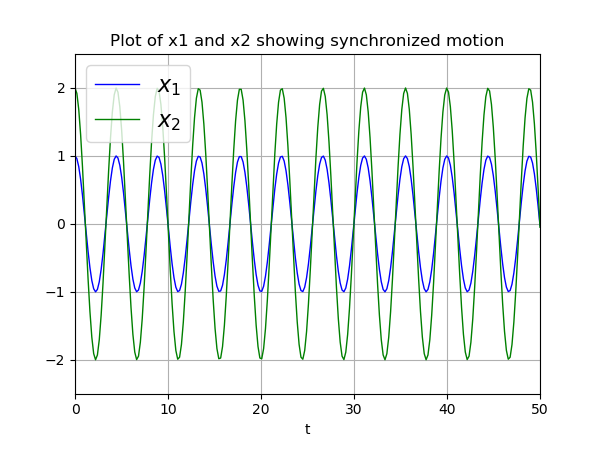
\includegraphics[width=6cm, height=6cm]{ej2_11.png}
\end{center}

\begin{verbatim}
# Plot the solution that was generated

import matplotlib.pyplot as plt
from numpy import loadtxt
from pylab import figure, plot, xlabel, grid, hold, legend, title, savefig, ylabel
from matplotlib.font_manager import FontProperties
% matplotlib inline

t, x1, y1, x2, y2, e1,e2 = loadtxt('ej2_1.dat', unpack=True)

figure(1, figsize=(6, 4.5))

xlabel('x')
ylabel('v')
grid(True)
#hold(True)
lw = 1
plt.xlim(-3,3)
plt.ylim (-3,3)

plot(x1, y1,'b', linewidth=lw)
plot(x2, y2, 'g', linewidth=lw)

legend((r'$x_1$', r'$x_2$'), prop=FontProperties(size=16))
title('Phase portrait for x1 and x2')
savefig('ej2_1.2.png', dpi=100)
\end{verbatim}

\begin{center}
  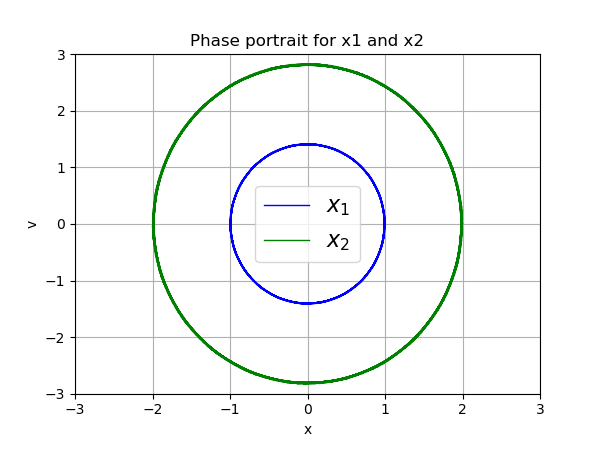
\includegraphics[width=6cm, height=6cm]{ej2_12.png}
\end{center}

\begin{verbatim}
#Plot the solution that was generated

import matplotlib.pyplot as plt
from numpy import loadtxt
from pylab import figure, plot, xlabel, grid, hold, legend, title, savefig, ylabel
from matplotlib.font_manager import FontProperties
% matplotlib inline

t, x1, xy, x2, y2, e1,e2 = loadtxt('ej2_1.dat', unpack=True)

figure(1, figsize=(6, 4.5))

xlabel('x1')
ylabel('x2')
grid(True)
#hold(True)
lw = 1
plt.xlim(-2,2)
plt.ylim (-2,2)

plot(x1,x2, 'b', linewidth=lw)
                                    
title('x1 versus x2')
savefig('ej2_1.3.png', dpi=100)

\end{verbatim}

\begin{center}
  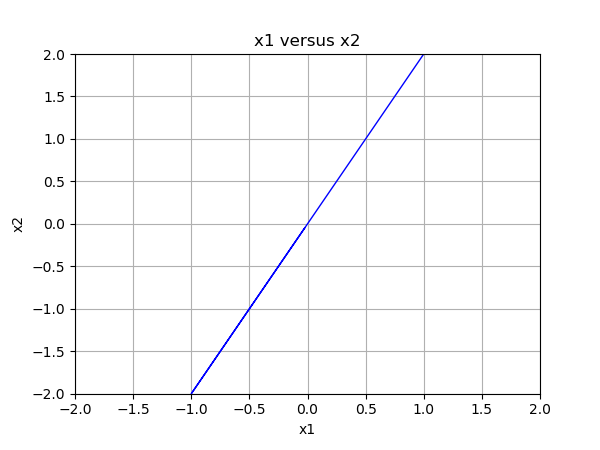
\includegraphics[width=6cm, height=6cm]{ej2_13.png}
\end{center}

\begin{verbatim}
#Plot the solution that was generated

from numpy import loadtxt
from pylab import figure, plot, xlabel, grid, hold, legend, title, savefig
from matplotlib.font_manager import FontProperties
%matplotlib inline

t, x1, y1, x2, y2, e1, e2 = loadtxt('ej2_1.dat', unpack=True)

figure(1, figsize=(6, 4.5))

xlabel('t')
grid(True)
#hold(True)
lw = 1

plot(t, e1, 'b', linewidth=lw)

plot(t, e2, 'g', linewidth=lw)

legend((r'$x_1$', r'$x_2$'), prop=FontProperties(size=16))
title('Relative Error of x1 and x2')
savefig('error2.1.png', dpi=100)

\end{verbatim}

\begin{center}
  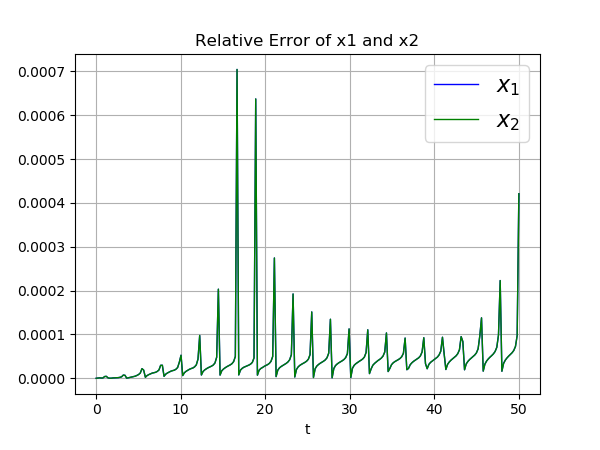
\includegraphics[width=6cm, height=6cm]{error21.png}
\end{center}


\subsection{Ejemplo 2.2}

En la siguiente se realizó lo dictado por el ejemplo 2.2 donde sólo se cambian los valores asociados a las variables y la ecuación a utilizar como se muestra a continuación:

\begin{verbatim}

# Parameter values
# Masses:
m1 = 1.0
m2 = 1.0
# Spring constants
k1 = 6.0
k2 = 4.0
# Natural lengths
L1 = 0.0
L2 = 0.0
# Friction coefficients
b1 = 0.0
b2 = 0.0

# Initial conditions
# x1 and x2 are the initial displacements; y1 and y2 are the initial velocities
x1 = -2.0
y1 = 0.0
x2 = 1.0
y2 = 0.0

# ODE solver parameters
abserr = 1.0e-8
relerr = 1.0e-6
stoptime = 25.0
numpoints = 250

# Create the time samples for the output of the ODE solver.
# I use a large number of points, only because I want to make
# a plot of the solution that looks nice.
t = [stoptime * float(i) / (numpoints - 1) for i in range(numpoints)]

# Pack up the parameters and initial conditions:
p = [m1, m2, k1, k2, L1, L2, b1, b2]
w0 = [x1, y1, x2, y2]

# Call the ODE solver.
wsol = odeint(vectorfield, w0, t, args=(p,),
              atol=abserr, rtol=relerr)

with open('ej2_2.dat', 'w') as f:
    # Print & save the solution.
    for t1, w1 in zip(t, wsol):
        print (t1, w1[0], w1[1], w1[2], w1[3],
               np.abs((w1[0]-(-2*np.cos(2*np.sqrt(3)*t1)))/(-2*np.cos(2*np.sqrt(3)*t1))), 
               np.abs((w1[2]-(np.cos(2*np.sqrt(3)*t1)))/(np.cos(2*np.sqrt(3)*t1))),
               file=f)
\end{verbatim}

La primera gráfica que se pide es la del comportamiento de los osciladores en una sola gráfica.


\begin{center}
  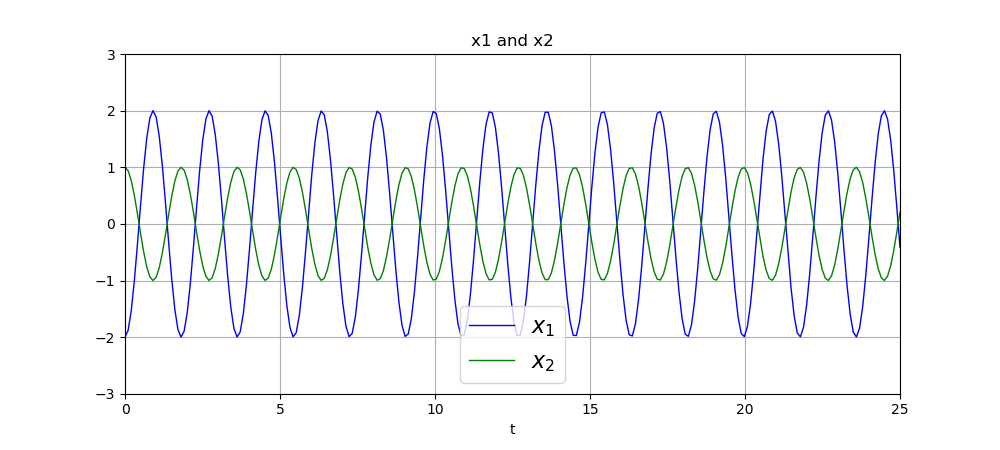
\includegraphics[width=6cm, height=6cm]{ej2_21.png}
\end{center}

En la siguiente se hace una de x1 vs x2 donde se aprecia que tienen en esencia un comportamiento muy parecido y, sobre todo, lineal. 

\begin{center}
  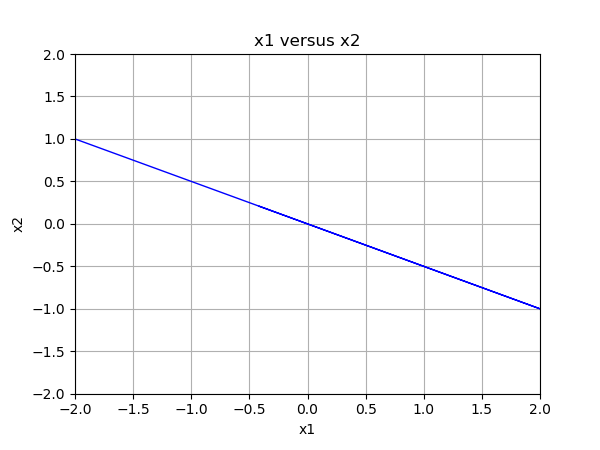
\includegraphics[width=6cm, height=6cm]{ej2_22.png}
\end{center}

Por último se ve el error cometido en la inferencia de sus valores
\begin{center}
  \includegraphics[width=6cm, height=6cm]{error22.png}
\end{center}

\subsection{Ejemplo 2.3}

En esta parte se hacen más gráficas, en total 6. Se vuelven a cambiar los valores de las variables involucradas y se ve cómo las condiciones iniciales sólo afectan a las amplitudes de cada uno

En las dos gráficas siguientes se observan las fases de cada oscilador.

\begin{center}
  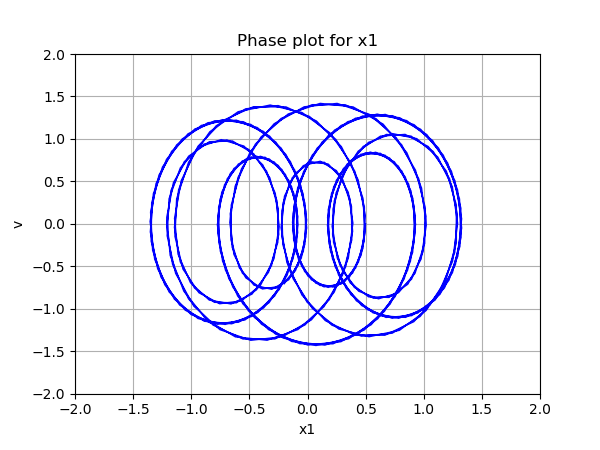
\includegraphics[width=6cm, height=6cm]{ej2_31.png}
\end{center}

\begin{center}
  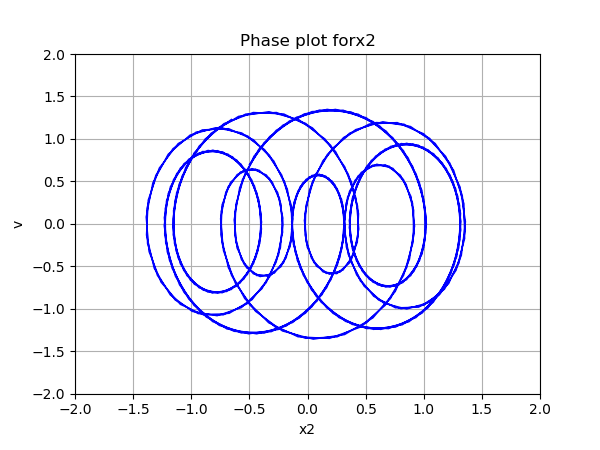
\includegraphics[width=6cm, height=6cm]{ej2_32.png}
\end{center}

Ahora se hace presencia de dos gráfica del desplazamiento que tuvieron los osciladores.
\begin{center}
  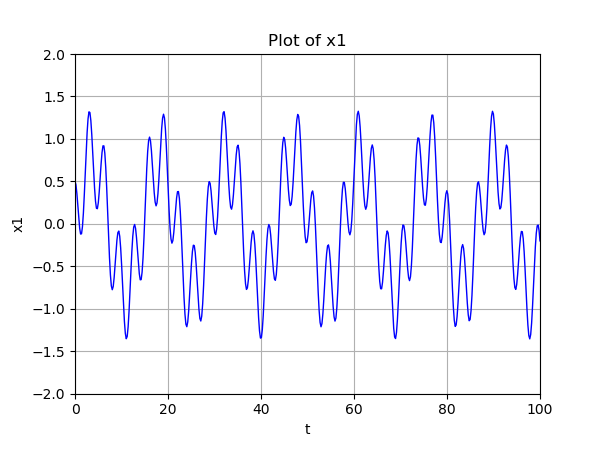
\includegraphics[width=6cm, height=6cm]{ej2_33.png}
\end{center}

\begin{center}
  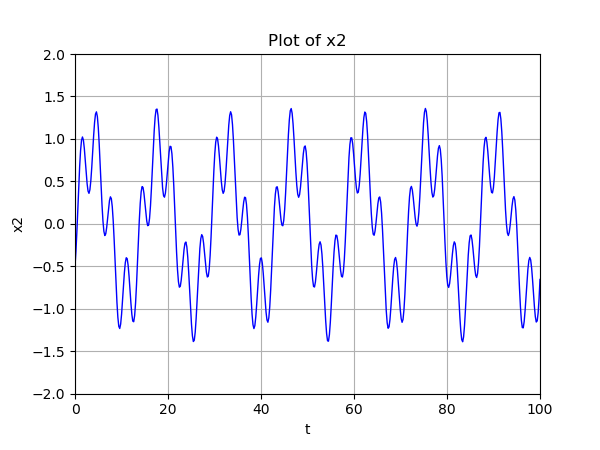
\includegraphics[width=6cm, height=6cm]{ej2_34.png}
\end{center}

Se hace una gráfica del comportamiento de los dos osciladores en una sola gráfica.
\begin{center}
  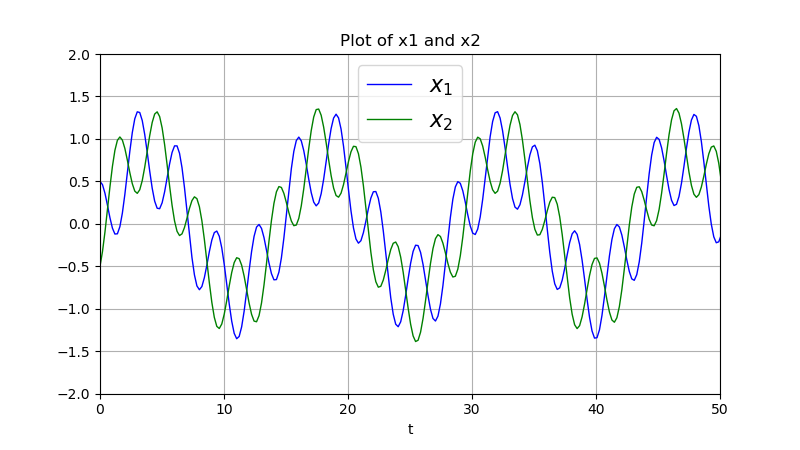
\includegraphics[width=6cm, height=6cm]{ej2_35.png}
\end{center}

Por último, se muestra una comparación directa entre los dos osciladores.
\begin{center}
  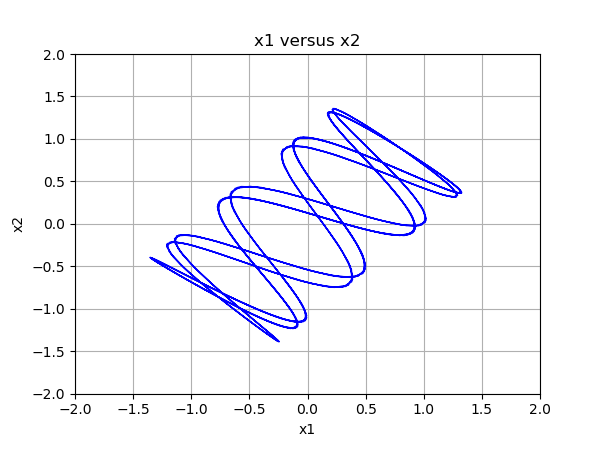
\includegraphics[width=6cm, height=6cm]{ej2_36.png}
\end{center}

\subsection{Ejemplo 2.4}

Con este ejemplo se nota un cambio, y es que los osciladores ya no tienen un comportamiento lineal como el observado en los ejemplos anteriores, es más errático e impredecible.

Se cambian los valores de las variables involucradas. Se hacen las mismas gráficas que en la actividad anterior pero el resultado no se asemeja mucho a lo visto anteriormente. 
\begin{center}
  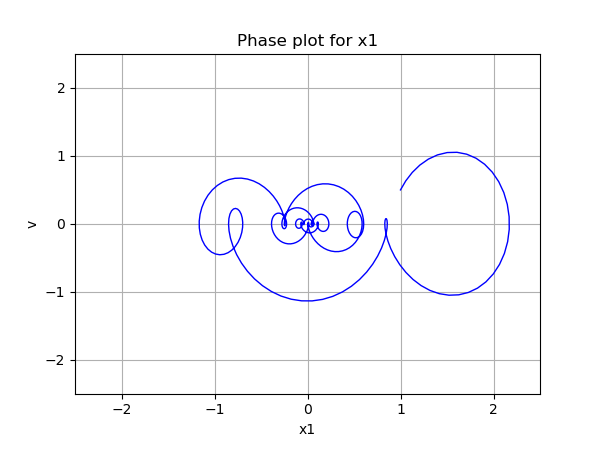
\includegraphics[width=6cm, height=6cm]{ej2_41.png}
\end{center}

\begin{center}
  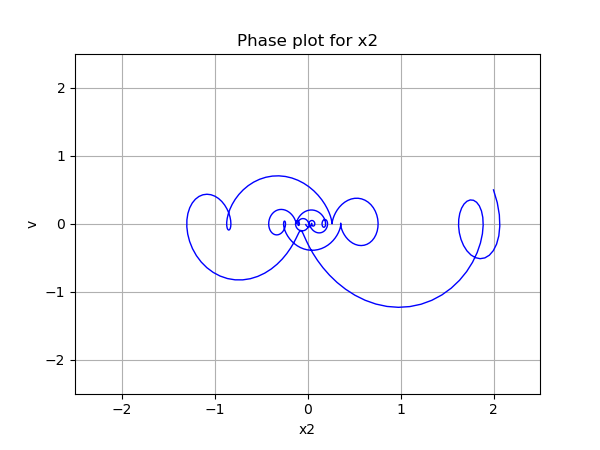
\includegraphics[width=6cm, height=6cm]{ej2_42.png}
\end{center}

\begin{center}
  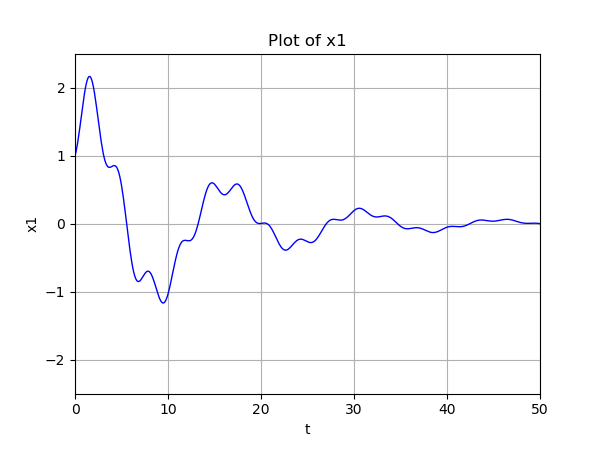
\includegraphics[width=6cm, height=6cm]{ej2_43.png}
\end{center}

\begin{center}
  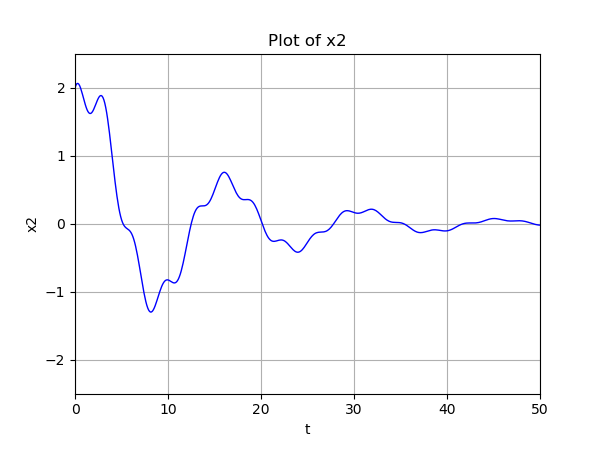
\includegraphics[width=6cm, height=6cm]{ej2_44.png}
\end{center}

\begin{center}
  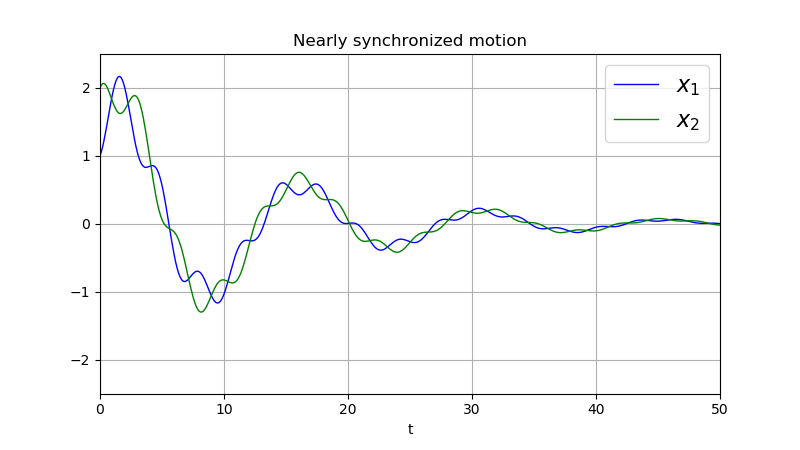
\includegraphics[width=6cm, height=6cm]{ej2_45.png}
\end{center}

\begin{center}
  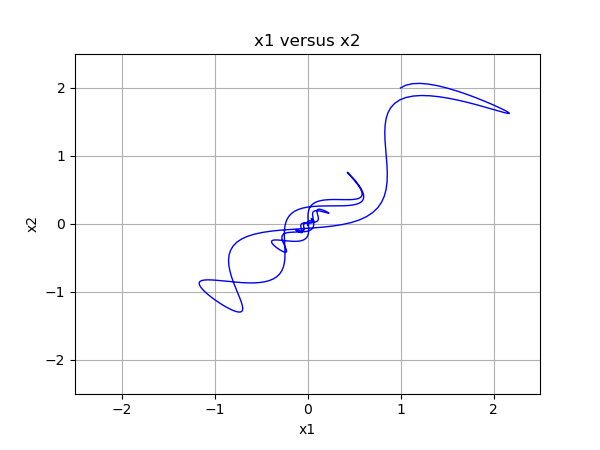
\includegraphics[width=6cm, height=6cm]{ej2_46.png}
\end{center}



\section{Apéndice}

1.- ¿En general te pareció interesante esta actividad de modelación matemática? ¿Qué te gustó mas? ¿Qué no te gustó?
\\
\\
Fue interesante, aprendí a que el lenguaje Python es útil al momento de recolectar datos y reproducirlos.
\\
\\
2.- La cantidad de material te pareció ¿bien?, ¿suficiente?, ¿demasiado?
\\
\\
Fue lo suficiente para entender el trasfondo de a lo que se quería llegar.
\\
\\
3.- ¿Cuál es tu primera impresión de Jupyter Lab? 
\\
\\
Un entorno amigable que presenta la misma estructura que Jupyter notebook.
\\
\\
4.- Respecto al uso de funciones de SciPy, ¿ya habías visto integración numérica en tus cursos anteriores? ¿Cuál es tu experiencia?.
\\
\\
En análiis numérico se vieron algunas técnicas, pero aquí es más rápido el realizarlas.
\\
\\
5.- El tema de sistema de masas acopladas con resortes, ¿ya lo habías resuelto en tu curso de Mecánica 2?  
\\
\\
Sí, pero se una manera diferente
\\
\\
6.- ¿Qué le quitarías o agregarías a esta actividad para hacerla más interesante y divertida?
\\
\\
Fue lo justo. está perfecta.
\end{document}
